\section{Persistent Data}
Collections will contain documents that belong to them. Such documents will then contain attributes to describe themselves and what they contain. This layout is depicted below in the same order and will be handled properly to be stored in Firebase.

\subsection{Users (Collection)}
\begin{itemize}
    \item User’s Authorization ID/Email (Document)
    \begin{itemize}
        \item Username: String
        \item User Logo: String
        \item Email: Boolean
        \item Google Email: Boolean
        \item Friends: Array of usernames
        \item Friend Requests: Array of usernames
        \item Games Played: Integer
        \item Games Won: Integer
        \item Bets: Array of past bets placed
    \end{itemize}
\end{itemize}

\subsection{Lobbies (Collection)}
\begin{itemize}
    \item Lobby ID (Document)
    \begin{itemize}
        \item Owner User ID: String (creator of the lobby)
        \item Lobby Type: String (can be public or private)
        \item Lobby Password: String (if it is private)
        \item Player Limit: Integer
        \item Players: Array (User IDs)
        \item AI Fill: Boolean (whether AI fills in for empty spots)
        \item Status: String (either open or closed)
        \item Betting Pool: Integer (collected bets for a game)
    \end{itemize}
\end{itemize}

\subsection{Friends (Collection)}
\begin{itemize}
    \item Friends List (Document)
    \begin{itemize}
        \item User ID: String (when requesting friends)
        \item Friend ID: String (recipient of friend request)
        \item Friends: Array
        \item Status: String (waiting, accepted, or declined)
    \end{itemize}
\end{itemize}

\subsection{Game Sessions (Collection)}
\begin{itemize}
    \item Game Session ID (Document)
    \begin{itemize}
        \item Lobby ID: String
        \item Players: Array (User IDs of players that are currently playing)
        \item Current Turn: String (username of the player who has an active turn)
        \item Deck: Integer (number of cards remaining in deck)
        \item Player Sets: Map (User ID should be connected to an array of completed sets)
        \item Game Status: String (ongoing or finished)
        \item Winner: String (username)
        \item Winner: String
        \item Prize Pool: Map (User ID of winner should be given the pooled money form bets)
    \end{itemize}
\end{itemize}

\subsection{Cards (Collection)}
\begin{itemize}
    \item Game Session (Document)
    \begin{itemize}
        \item Game Session ID: String
        \item Deck: Array (of Cards)
        \item Player Hand: Map (connecting a User ID to a unique array of cards)
    \end{itemize}
\end{itemize}

\subsection{Bets (Collection)}
\begin{itemize}
    \item Game Session (Document)
    \begin{itemize}
        \item Players: Array (of players involved in the bet)
        \item Total: Integer (of the finalized pool)
        \item Winner: String (User who won, prize mapped to their account and info)
    \end{itemize}
\end{itemize}

\subsection{Shop (Collection)}
\begin{itemize}
    \item Item (Document)
    \begin{itemize}
        \item Item Name: String
        \item Item Pic: String (hardcoded link to show the image)
        \item Price: Integer
        \item Featured: Boolean (for weekly new limited edition items)
    \end{itemize}
\end{itemize}

\begin{center}
    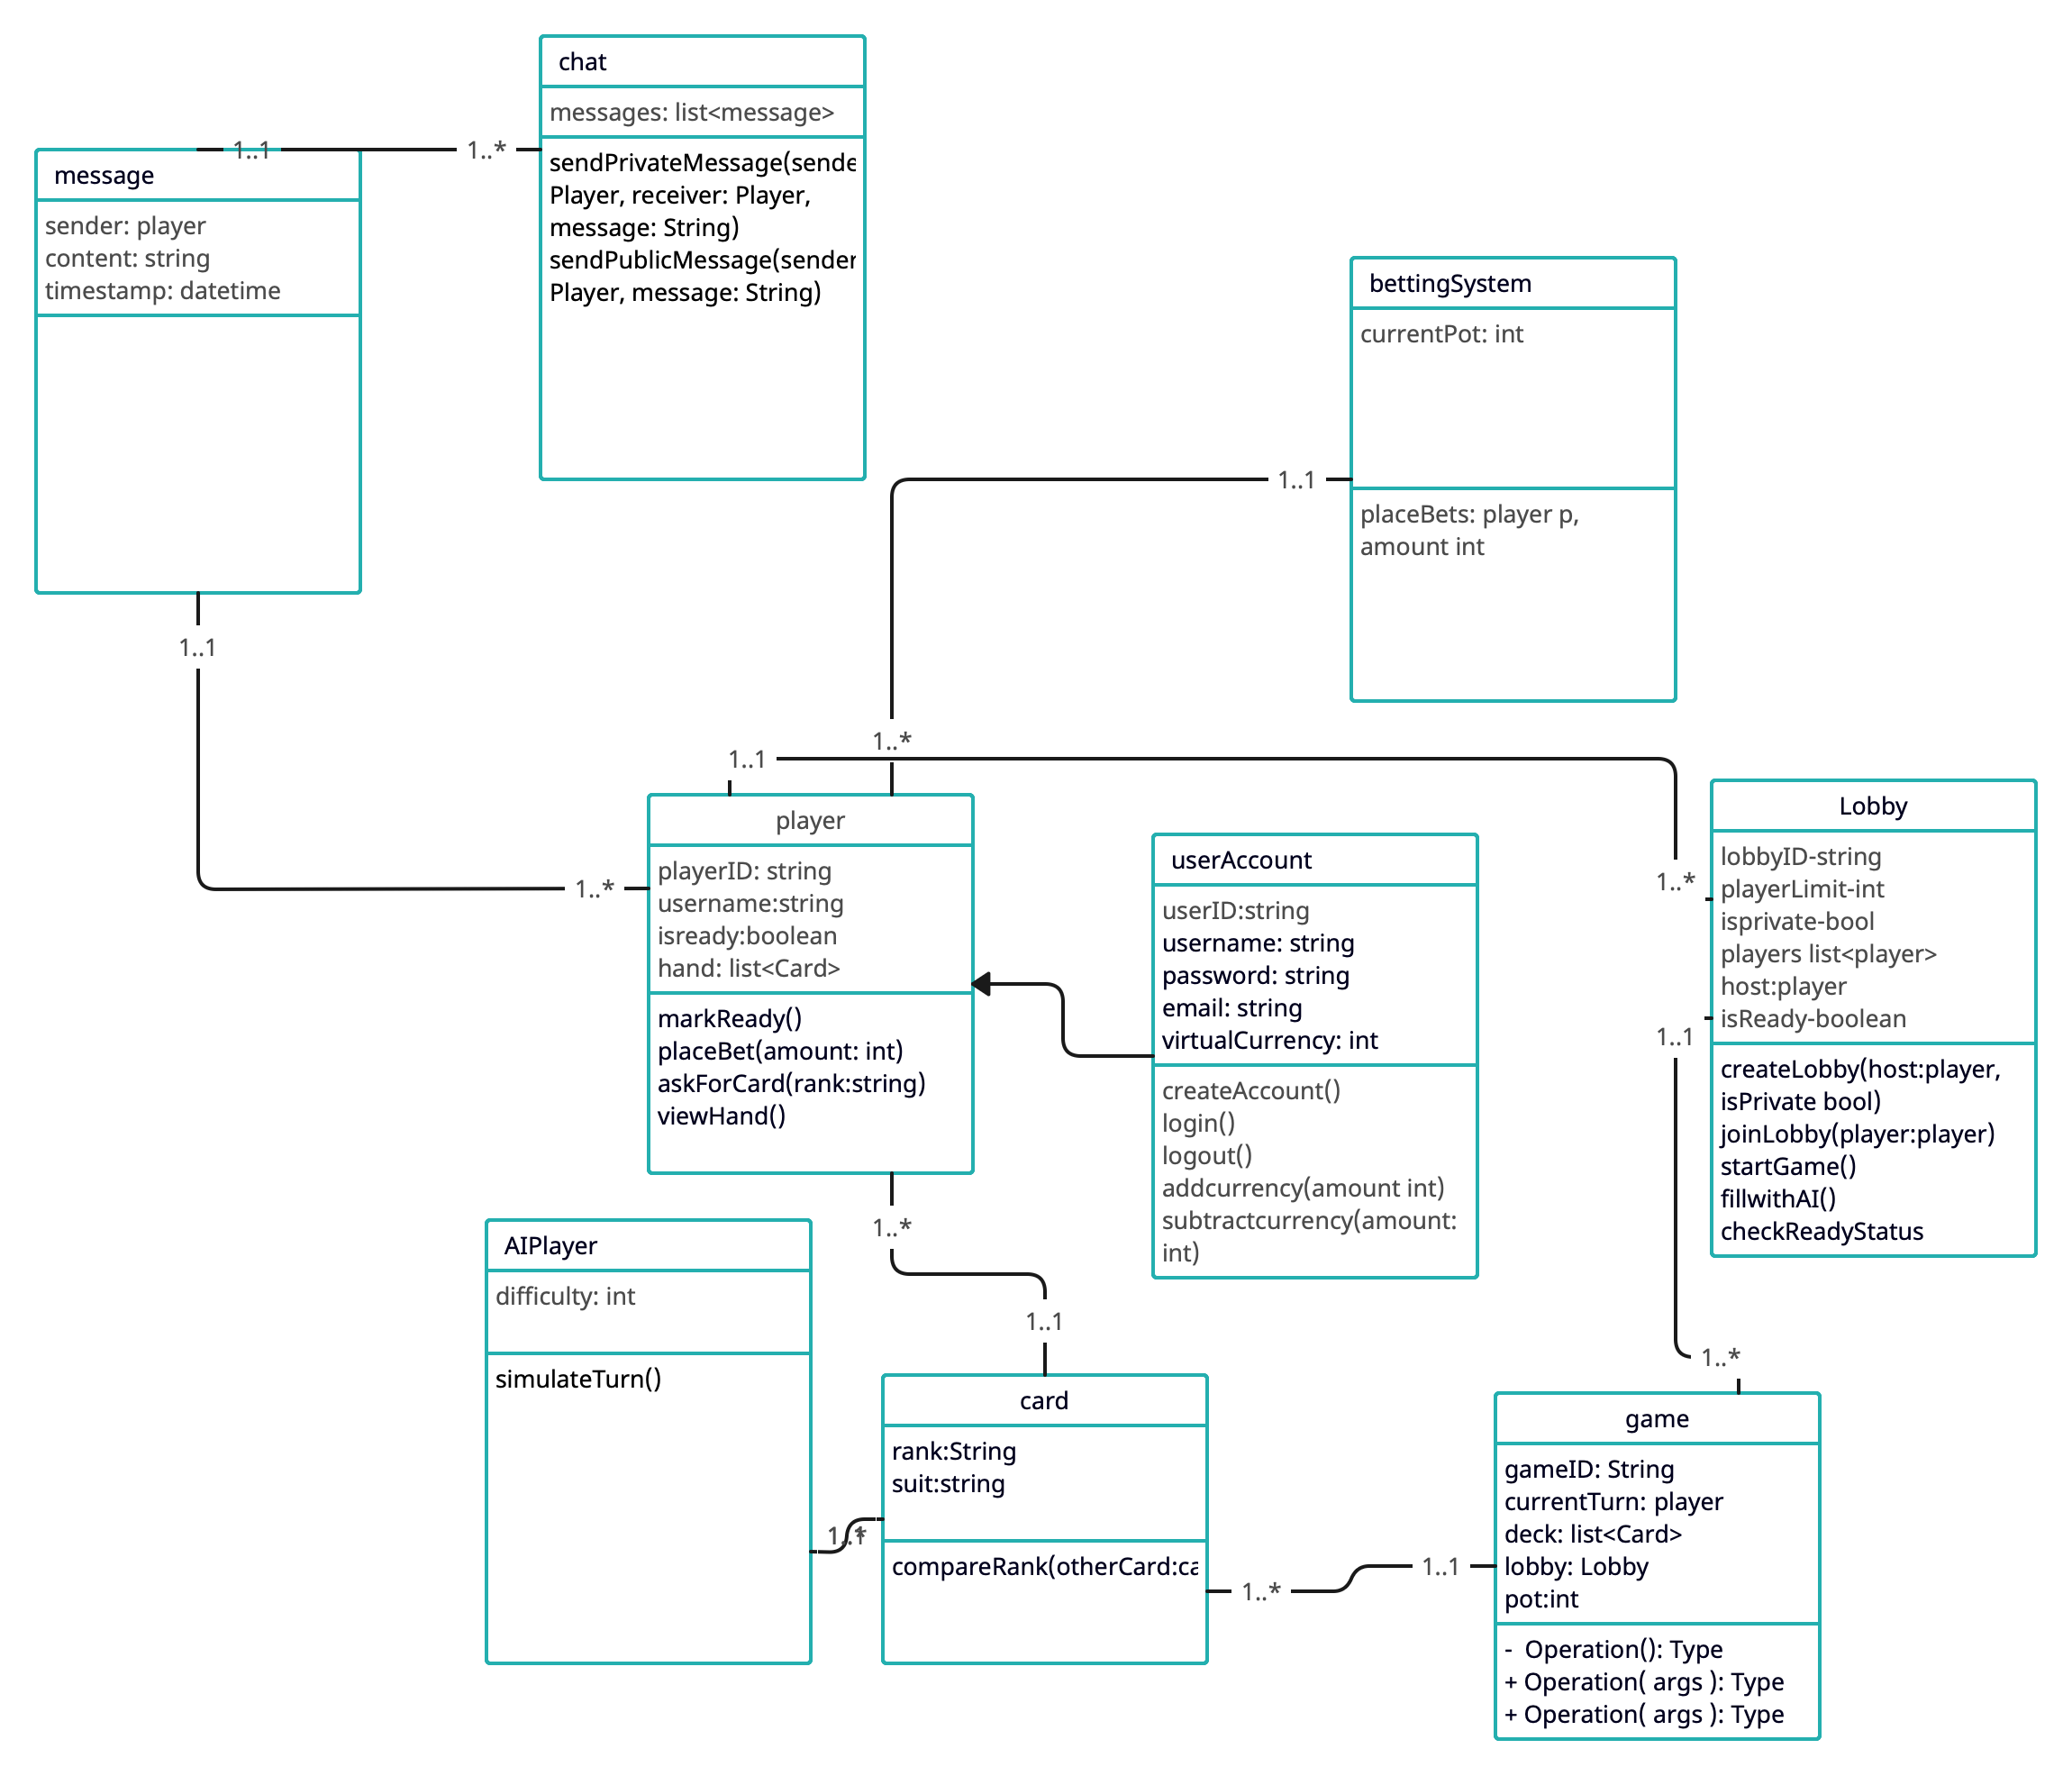
\includegraphics[scale=0.2]{uml_diagram.png}
\end{center}
In this UML diagram, we outline the architecture of our Go Fish card game application, which integrates several key components. At the center, the player class handles user actions such as betting, viewing their hand, and interacting with the bettingSystem. We’ve designed the Lobby to manage game sessions, enabling players to join, start games, and interact with one another through the chat system. Additionally, the AIPlayer class simulates opponent behavior with varying difficulty levels. Our design also supports account management via the userAccount class, allowing players to log in, manage their virtual currency, and participate in games.